\documentclass{beamer}  
\usetheme{Warsaw}
\title{Introduction to AI and ML}
\subtitle{Matrix Project}
\author{Manideep, EE17BTECH11046 \\ Yashas, ES17BTECH11025}
\begin{document}

\begin{frame}

\titlepage
 
\end{frame}  

\begin{frame}[t]{Question:Q71 of JEE Main 2013(Code P)}
\vspace{5em}
The circle passing through (1,-2) and touching the axis of x at (3,0) also passes through the point:

\vspace{1.5em}
\hspace{1.5em} a)(-5,2) \hspace{1.5em} b)(2,-5) \hspace{1.5em} c)(5,-2) \hspace{1.5em} d)(-2,5)
\vspace{1.5em}
\end{frame}

\begin{frame}[t]{Matrix form of the question}
\vspace{5em}
The circle passing through
$
\begin{bmatrix}
1\\
-2
\end{bmatrix}$
and touching the axis of x at
$
\begin{bmatrix}
3\\
0
\end{bmatrix}$
also passes through the point:
\begin{columns}[onlytextwidth]
\column{0.25\textwidth}
\[
1)\begin{bmatrix}
-5\\
2
\end{bmatrix}\]
\column{0.25\textwidth}
\[2)\begin{bmatrix}
2\\
-5
\end{bmatrix}\] 
\column{0.25\textwidth}
\[3)\begin{bmatrix}
5\\
-2
\end{bmatrix}\] 
\column{0.25\textwidth}
\[4)\begin{bmatrix}
-2\\
5
\end{bmatrix} 
\]
\end{columns}
\end{frame}

\begin{frame}{Figure 1}
\begin{center}
\vspace{-0.75em}
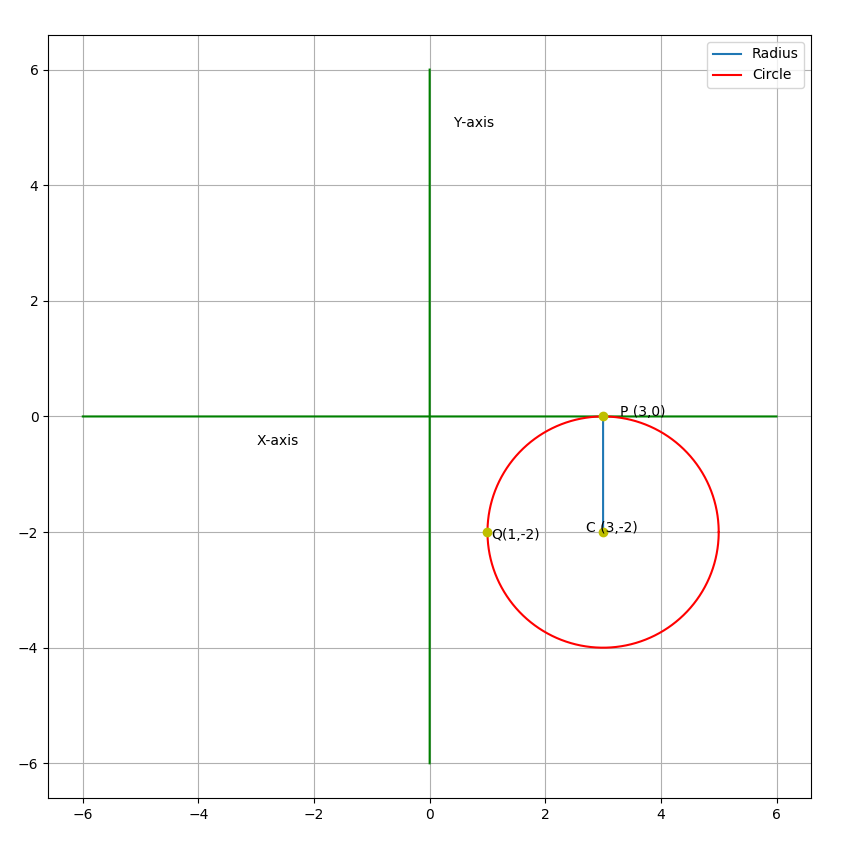
\includegraphics[scale=0.39]{Fig_Circle1.png}
\end{center}
\end{frame}

\begin{frame}{Solution}
\vspace{2em}
As x-axis is tangent to circle at 
$
\begin{bmatrix}
3\\
0
\end{bmatrix}$
,\\
Also we know, if PQ $\perp$ AB, $(P-Q)^T(A-B) = 0$,thus
\[
\begin{bmatrix}
k & 0
\end{bmatrix} 
(\boldsymbol{C} -
\begin{bmatrix}
3\\
0
\end{bmatrix}
) = 0 
\]
\[
\begin{bmatrix}
1 & 0
\end{bmatrix} 
\boldsymbol{C} = 
\begin{bmatrix}
1 & 0
\end{bmatrix}
\begin{bmatrix}
3\\
0
\end{bmatrix}  
\]
\\
\[
\hspace{12em}
\begin{bmatrix}
1 & 0
\end{bmatrix} 
\boldsymbol{C} = 
3
\hspace{10em} (1)
\]
\end{frame}

\begin{frame}
As standard form of circle in matrix form is:
\[
||\boldsymbol{x-C}||^2=r^2
\]
\[
\boldsymbol{x^Tx}-2\boldsymbol{C^Tx} = r^2 - \boldsymbol{C^TC}
\]
Given,$\begin{bmatrix}
3 & 0
\end{bmatrix}$
and
$\begin{bmatrix}
1 & -2
\end{bmatrix}$
lie of the circle,
\[
\hspace{6em}
\begin{bmatrix}
3 & 0
\end{bmatrix}
\begin{bmatrix}
3\\
0
\end{bmatrix}
-2\boldsymbol{C^T}
\begin{bmatrix}
3\\
0
\end{bmatrix}
=r^2 - \boldsymbol{C^TC}
\hspace{7em} (2)
\]
\[
\hspace{6em}
\begin{bmatrix}
1 & -2
\end{bmatrix}
\begin{bmatrix}
1\\
-2
\end{bmatrix}
-2\boldsymbol{C^T}
\begin{bmatrix}
1\\
-2
\end{bmatrix}
=r^2 - \boldsymbol{C^TC}
\hspace{4em} (3)
\]
From above two equations:
\[
9-2\boldsymbol{C^T}
\begin{bmatrix}
3\\
0
\end{bmatrix}
=
5 -2\boldsymbol{C^T}
\begin{bmatrix}
1\\
-2
\end{bmatrix}
\]
\[
\hspace{7em}
\boldsymbol{C^T}
\begin{bmatrix}
1\\
1
\end{bmatrix}
 = 1
 \hspace{1em} or 
 \hspace{1em}
 \begin{bmatrix}
1 & 1
\end{bmatrix}
\boldsymbol{C}
 = 1
 \hspace{6em} (4)
\]
\end{frame}

\begin{frame}
From equations (1) and (4):
\[
\begin{bmatrix}
1 & 1\\
1 & 0
\end{bmatrix}
\boldsymbol{C} = 
\begin{bmatrix}
1\\
3
\end{bmatrix}
\]
Using elementary transformations on augmented matrix:
\[
\begin{bmatrix}
1 & 1 & 1\\
1 & 0 & 3
\end{bmatrix}
\leftrightarrow
\begin{bmatrix}
1 & 1 & 1\\
0 & -1 & 2
\end{bmatrix}
\leftrightarrow
\begin{bmatrix}
1 & 0 & 3\\
0 & -1 & 2
\end{bmatrix}
\leftrightarrow
\begin{bmatrix}
1 & 0 & 3\\
0 & 1 & -2
\end{bmatrix}
\]
Then
\[
\boldsymbol{C} =
\begin{bmatrix}
3\\
-2
\end{bmatrix}
\]
\end{frame}
\begin{frame}
Substituting the value of $\boldsymbol{C}$ in equation 2:
\[
9 - 2
\begin{bmatrix}
3 & -2
\end{bmatrix}
\begin{bmatrix}
3\\
0
\end{bmatrix}
 = r^2 - 
\begin{bmatrix}
3 & -2
\end{bmatrix}
\begin{bmatrix}
3\\
-2
\end{bmatrix}
\]
\[
r=2
\]
So,the equation of circle becomes:
\[
||\boldsymbol{x} - 
\begin{bmatrix}
3\\
-2
\end{bmatrix}
||^2 = 4
\]
Clearly,the only point satisfying the circle equation is:
$\begin{bmatrix}
5\\
-2
\end{bmatrix}$

\end{frame}

\begin{frame}{Figure 2}
\begin{center}
\vspace{-0.75em}
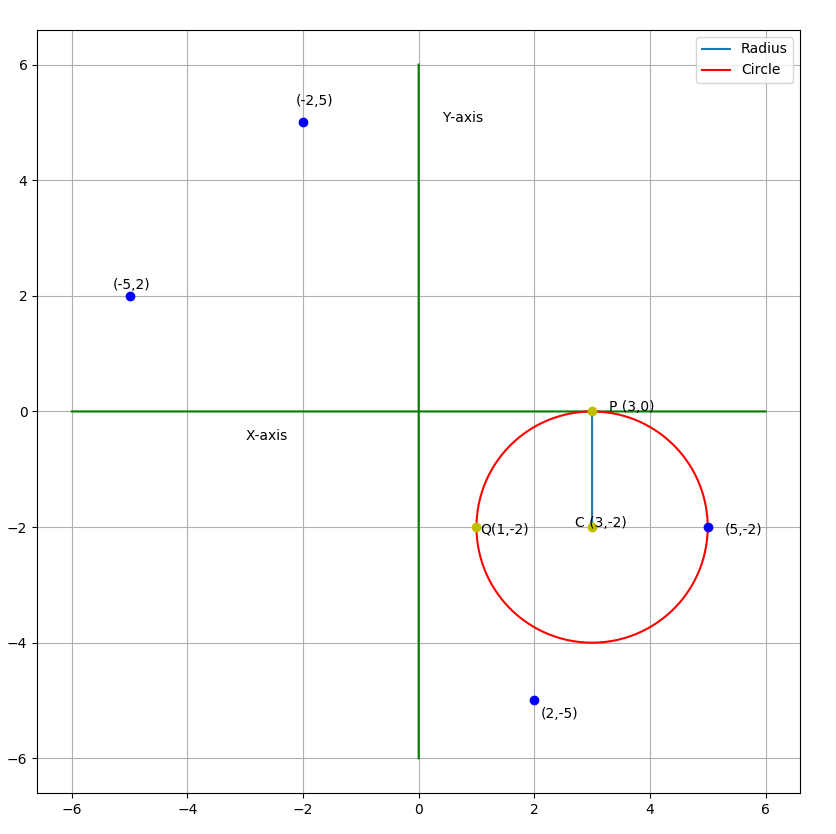
\includegraphics[scale=0.39]{Fig_Circle2.png}
\end{center}
\end{frame}

\end{document}